% !TEX program = lualatex
%% SHINE 2026 poster -- Toward a Dynamic Chromosphere for AWSoM-R
%% Template: 2025 SHINE Gemini/UM beamerposter (Sokolov & Gombosi testbed kit)
%% Size: 36 in x 48 in PORTRAIT.  Content mirrors the web poster (web/index.html).
%%
%% BUILD (must use LuaLaTeX -- the gemini theme loads Raleway/Lato via fontspec
%% from the TeX-Live tree, which XeLaTeX/fontconfig does not see by name):
%%   latexmk poster.tex            (run from docs/poster-shine/)
%% The local .latexmkrc is the recipe: it pins $out_dir = latex-build/ and
%% $pdf_mode = lualatex, so build files ALWAYS land in latex-build/ -- no
%% -output-directory or -lualatex flag needed.
%% In VS Code (LaTeX Workshop): just build -- the `% !TEX program` line above
%% selects lualatex and .vscode/settings.json sends output to latex-build/.
%%
\documentclass[final, dvipsnames, 20pt]{beamer}

% ====================
% Packages
% ====================
\usepackage[T1]{fontenc}
\usepackage{lmodern}
\usepackage{anyfontsize}
\usepackage[size=custom,width=3,height=4,scale=0.82]{beamerposter}
\setlength{\paperwidth}{36in}
\setlength{\paperheight}{48in}
\usepackage{xcolor}

\usetheme{gemini}
\usecolortheme{UM}

\usepackage{graphicx}
\usepackage{booktabs}
\usepackage{amsmath}
\usepackage{amssymb}
\usepackage{mdframed}
\usepackage{paralist}
\usepackage{url}
\usepackage[font=small]{caption}
\usepackage{multicol}

% ====================
% Bibliography (biblatex + biber; latexmk runs biber automatically)
% Author-year, compact "(Author Year)" inline, titles suppressed in the list.
% ====================
\usepackage[backend=biber, style=authoryear,
            maxbibnames=2, minbibnames=1, maxcitenames=2, mincitenames=1,
            giveninits=true, uniquename=false, uniquelist=false,
            doi=false, isbn=false, url=false, eprint=false, dashed=false,
            natbib=true]{biblatex}
\addbibresource{references.bib}
\renewcommand*{\nameyeardelim}{\addspace}      % "Author Year", no comma
\renewcommand*{\finalnamedelim}{\addspace\&\addspace}  % "A & B", not "A and B"
\renewbibmacro*{in:}{}                          % drop "In:" before journal
\AtEveryBibitem{\clearfield{title}\clearfield{number}\clearfield{note}}
\renewcommand*{\bibfont}{\scriptsize}
\setbeamertemplate{bibliography item}{}         % no beamer bib icon
\setlength{\bibitemsep}{0pt plus 1pt}
\setlength{\bibhang}{1em}

\graphicspath{{figs/}}

% ====================
% Lengths -- 3 columns:  (N+1)*sep + N*col = paperwidth
% 4*0.5in + 3*11.35in = 2in + 34.05in = 36.05in
% ====================
\newlength{\sepwidth}
\newlength{\colwidth}
\setlength{\sepwidth}{0.5in}
\setlength{\colwidth}{11.35in}
\newcommand{\separatorcolumn}{\begin{column}{\sepwidth}\end{column}}

% ====================
% Title / authors
% ====================
\title{Toward a Dynamic Chromosphere for AWSoM-R\\[0.45ex]
  {\fontsize{42}{50}\selectfont\color{Maize}\mdseries
   A Field-Aligned Two-Fluid Model of Ionization \& Chromospheric Evaporation}}
\newcommand{\authmail}[1]{\,{\fontsize{19}{22}\selectfont\mdseries\color{Maize}\texttt{#1}}}
\author[Zhu et al.]{\fontsize{29}{34}\selectfont
  Keheng Zhu\authmail{zkeheng@umich.edu}\quad
  Xianyu Liu\authmail{xianyu@umich.edu}\quad
  Igor Sokolov\authmail{igorsok@umich.edu}\quad
  Lulu Zhao\authmail{zhlulu@umich.edu}}
\institute[U.\ Michigan]{University of Michigan, Climate \& Space Sciences and Engineering, Ann Arbor, MI, USA}

\footercontent{\insertshortauthor \hfill SHINE 2026 \hfill \insertshortinstitute}

% Maize-on-transparent logos sit cleanly on the dark-blue Gemini header
\logoleft{
\includegraphics[width=11cm]{logos/block_m-hex}}
\logoright{
\includegraphics[width=13cm]{logos/CLEAR_logo_maze}}

% ====================
% Content helpers
% ====================
\newcommand{\mz}[1]{{\color{Blue}\textbf{#1}}}     % UM-blue emphasis (web .mz)
\newcommand{\rd}[1]{{\color{TappanRed}\textbf{#1}}} % red emphasis     (web .rd)

% Highlight call-out (web .hl): light-blue panel with a blue left rule
\newmdenv[
  backgroundcolor=Blue!8, linecolor=Blue, linewidth=5pt,
  topline=false, rightline=false, bottomline=false, leftline=true,
  innerleftmargin=10pt, innerrightmargin=10pt,
  innertopmargin=7pt, innerbottommargin=7pt,
  skipabove=6pt, skipbelow=6pt,
]{hlbox}

% Equation panel (web .eq): soft maize box
\newmdenv[
  backgroundcolor=Maize!12, linecolor=Maize!72!black, linewidth=1.5pt,
  roundcorner=6pt,
  innerleftmargin=8pt, innerrightmargin=8pt,
  innertopmargin=7pt, innerbottommargin=7pt,
  skipabove=6pt, skipbelow=6pt,
]{eqbox}

% Compact figure caption matching the web (bold lead-in, no float number)
\newcommand{\figcap}[1]{\par\vspace{0.4ex}{\footnotesize\color{black!75} #1}}

% Spectroscopic ion labels in true small-caps (Lato has none -> borrow Latin Modern)
\newcommand{\ion}[2]{#1\,{\rmfamily\textsc{#2}}}

% Fully-bold table value (bold text AND bold math digits)
\newcommand{\evap}[1]{{\bfseries\boldmath #1}}

\begin{document}
\input{newcommands_all}
\setbeamercolor{background canvas}{bg=white}

\begin{frame}[t]
\begin{columns}[t]
\separatorcolumn

%%=====================================================================
%%  COLUMN 1
%%=====================================================================
\begin{column}{\colwidth}

\begin{block}{Why the chromosphere?}
\begin{hlbox}
The chromosphere is the \mz{partially-ionized gateway} that sets the mass \& energy
fed to the corona and solar wind --- yet global models \rd{prescribe} it rather than
solve it.
\end{hlbox}
\begin{compactitem}
  \item $6$\,kK $\to$ $>$$1$\,MK across a few thousand km; density drops by orders of magnitude.
  \item Processes nearly all of the plasma \& Poynting flux that fill the corona ---
        via evaporation, spicules, wave heating.
\end{compactitem}
\begin{center}
  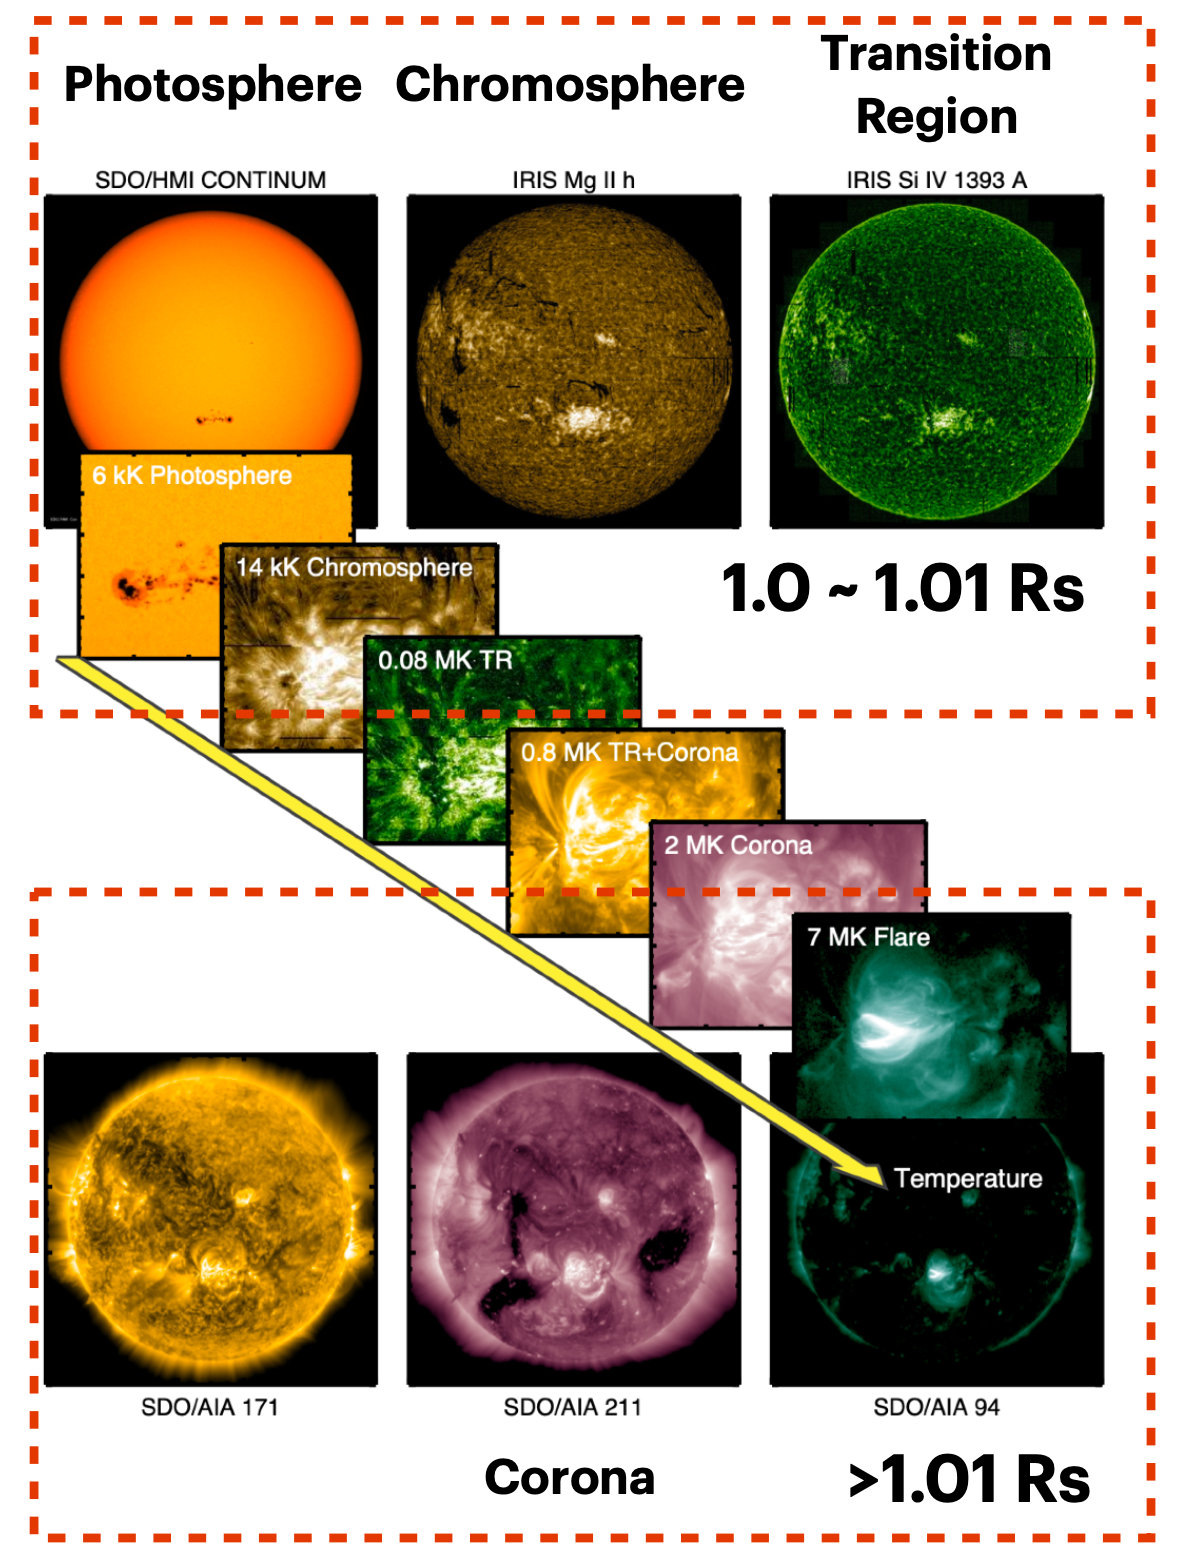
\includegraphics[width=0.66\linewidth]{intro_atmos_obs.png}
\end{center}
\figcap{\textbf{Layers of the solar atmosphere} in SDO/AIA \& IRIS passbands --- $6$\,kK
  photosphere $\to$ chromosphere $\to$ transition region $\to$ $>$$1$\,MK corona.}
\end{block}

\begin{block}{AWSoM-R's missing lower boundary}
\mz{AWSoM / AWSoM-R}~\parencite{vanderHolst2014,Sokolov2021} places its inner boundary in the upper chromosphere and injects
Alfv\'en-wave Poynting flux through a thin, quasi-static layer. The dynamic chromosphere
below is replaced by crude BCs:
\begin{compactitem}
  \item temperature fixed at unrealistic \rd{$T\!\sim\!5\times10^{4}$\,K};
  \item electron density far below chromospheric, $n_e\!\sim\!2\times10^{17}$\,m$^{-3}$;
  \item plasma speed \rd{left unspecified}.
\end{compactitem}
\begin{hlbox}
\mz{Chromospheric evaporation} --- conduction-driven upflows --- governs the real
mass/energy exchange; it must be \rd{solved, coupled to the corona}.
\end{hlbox}
\begin{center}
  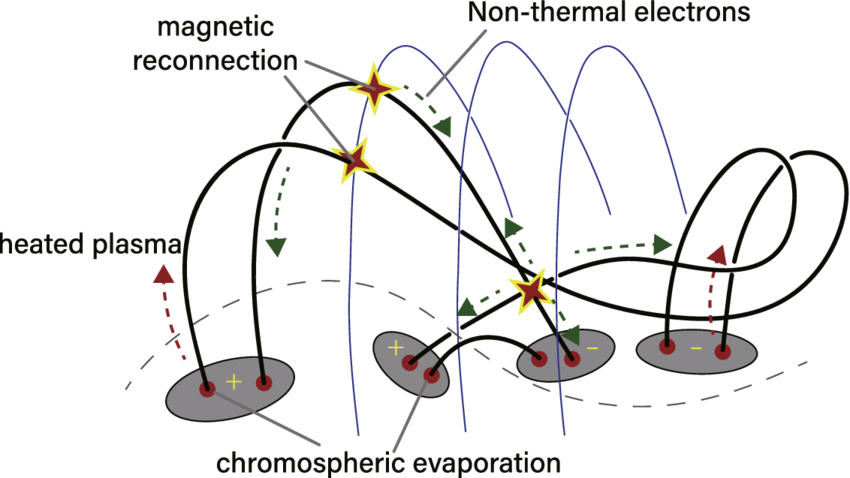
\includegraphics[width=0.82\linewidth]{intro_evaporation.png}
\end{center}
\figcap{\textbf{Flare/CME reconnection} drives non-thermal electrons \& downward conduction
  into the footpoints; the heated chromosphere \emph{evaporates}, feeding hot plasma upward.}
\end{block}

\begin{block}{From 3D MHD to a 1.5D field-aligned model}
\begin{compactitem}
  \item \mz{Two assumptions:} the flow is field-aligned, $\mathbf V\parallel\mathbf B$,
        and the field is static, $\partial\mathbf B/\partial t=0$ --- so a fixed (PFSS)
        potential field serves as a \mz{geometric guide}.
  \item Split into flux tubes of cross-section $A(s)\propto 1/B(s)$; derivatives
        reduce to $\partial/\partial s$.
  \item The \rd{$B$ field enters purely as an area factor}.
  \item 13-variable 3D MHD $\to$ \mz{6 field-aligned variables}.
\end{compactitem}
\begin{center}
  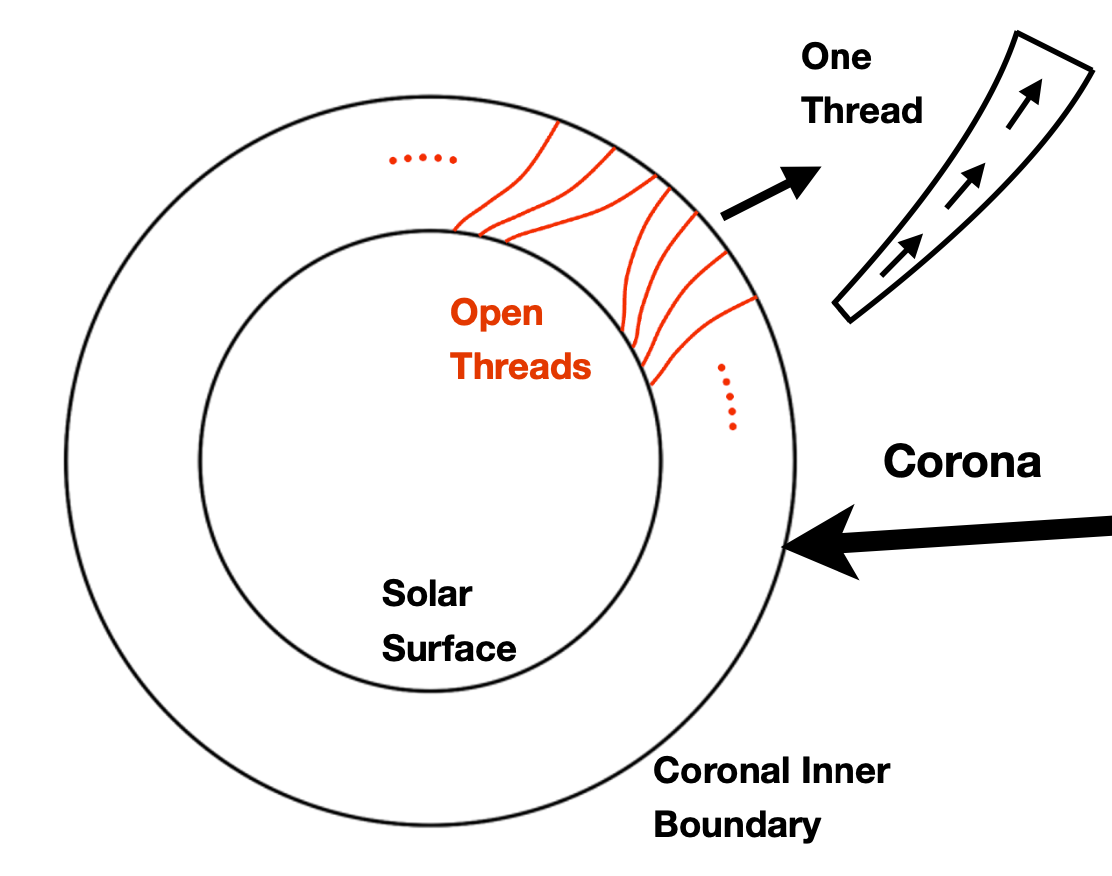
\includegraphics[width=0.88\linewidth]{geom_threads.png}
\end{center}
\figcap{\textbf{Open/closed field threads} $\to$ independent flux tubes; the problem
  becomes gas flow along one tube.}
\end{block}

\end{column}
\separatorcolumn

%%=====================================================================
%%  COLUMN 2
%%=====================================================================
\begin{column}{\colwidth}

\begin{block}{Two-fluid field-aligned equations}
Conservative form (ions $i$ + neutrals $n$; electrons folded in by quasi-neutrality):
\begin{eqbox}
\centering
$\dfrac{\partial \mathbf U}{\partial t}
  + B\,\dfrac{\partial}{\partial s}\!\left(\dfrac{\mathbf F}{B}\right)=\mathbf S$
\\[1.6ex]
\resizebox{0.99\linewidth}{!}{$
\mathbf U=\begin{bmatrix}\rho_i\\\rho_n\\\rho_iV\\\rho_nU\\e_i\\e_n\end{bmatrix}\!,\;
\mathbf F=\begin{bmatrix}\rho_iV\\\rho_nU\\\rho_iV^2+2n_ik_BT_i\\\rho_nU^2+n_nk_BT_n\\
   (e_i+2n_ik_BT_i)V\\(e_n+n_nk_BT_n)U\end{bmatrix}\!,\;
\mathbf S=\begin{bmatrix}+\Gamma\\-\Gamma\\-\rho_i g+a_i+R\\-\rho_n g+a_n-R\\
   -\rho_i gV+Q_i\\-\rho_n gU+Q_n\end{bmatrix}
$}
\end{eqbox}
Electron pressure $p_e=n_ik_BT_e$ enters $e_i$ via the factor 2. The \textbf{source
$\mathbf S$} couples the fluids and the corona:
\begin{compactitem}
  \item $\Gamma$ --- net \textbf{ionization} mass exchange (neutral$\to$ion;
        \citeauthor{Voronov1997}, \citeauthor{Hummer1994} rates);
  \item $a_s=p_sB\,\partial_s(1/B)$ --- flux-tube \textbf{area} force; $g$ field-aligned gravity;
  \item $R=\rho_i\nu_{in}(U-V)+\Gamma U$ --- ion--neutral \textbf{drag} + ionization momentum;
  \item $Q_i,Q_n$ --- frictional + $T_i$--$T_n$ collisional \textbf{exchange}, conduction
        $-\partial_s q$, ionization cost, radiative \textbf{cooling}.
\end{compactitem}
\end{block}

\begin{block}{Source physics (calibrated to Model C7)}
\mz{Non-equilibrium H ionization / recombination} --- five channels integrated dynamically:
\begin{compactitem}
  \item collisional $S_i$ \parencite{Voronov1997};
  \item multilevel collisional $S_{\mathrm{CR}}$ (detailed balance);
  \item radiative recomb.\ \parencite{Hummer1994} $\alpha_r\propto T_e^{-0.75}$;
  \item three-body $\alpha_c\propto n_e\,(k_BT_e)^{-9/2}$ \parencite{HinnovHirschberg1962};
  \item photoionization $P_\mathrm{phot}$ --- a \mz{frozen radiative-rate} closure
        \parencite{Sollum1999,CarlssonStein2002}: the slowly-varying photoionizing field
        freezes $P_\mathrm{phot}$ to a function of height, fixed by inverting C7
        ionization equilibrium.
\end{compactitem}
\textbf{Radiative cooling:} opt-thick \ion{H}{i}/\ion{Ca}{ii}/\ion{Mg}{ii}
\parencite{CarlssonLeenaarts2012} + opt-thin $n_en_H\Lambda(T)$.
\textbf{Conduction:} electron (Spitzer, with $e$--$n$ collisions in the denominator) +
neutral (kinetic-theory) closures:
\begin{eqbox}
\centering
\resizebox{0.985\linewidth}{!}{$
\kappa_e=\dfrac{9.2048\times10^{-12}\,n_e\,T_e^{5/2}}
              {n_e+2.836\times10^{-11}\,n_n\,T_e^{2}},
\qquad
\kappa_n=\dfrac{0.0342\,n_n\,T_n}
              {1.206\,n_i\sqrt{T_n+T_i}+1.706\,n_n\sqrt{T_n}}
\;\;[\mathrm{W\,m^{-1}K^{-1}}]
$}
\end{eqbox}
\begin{center}
  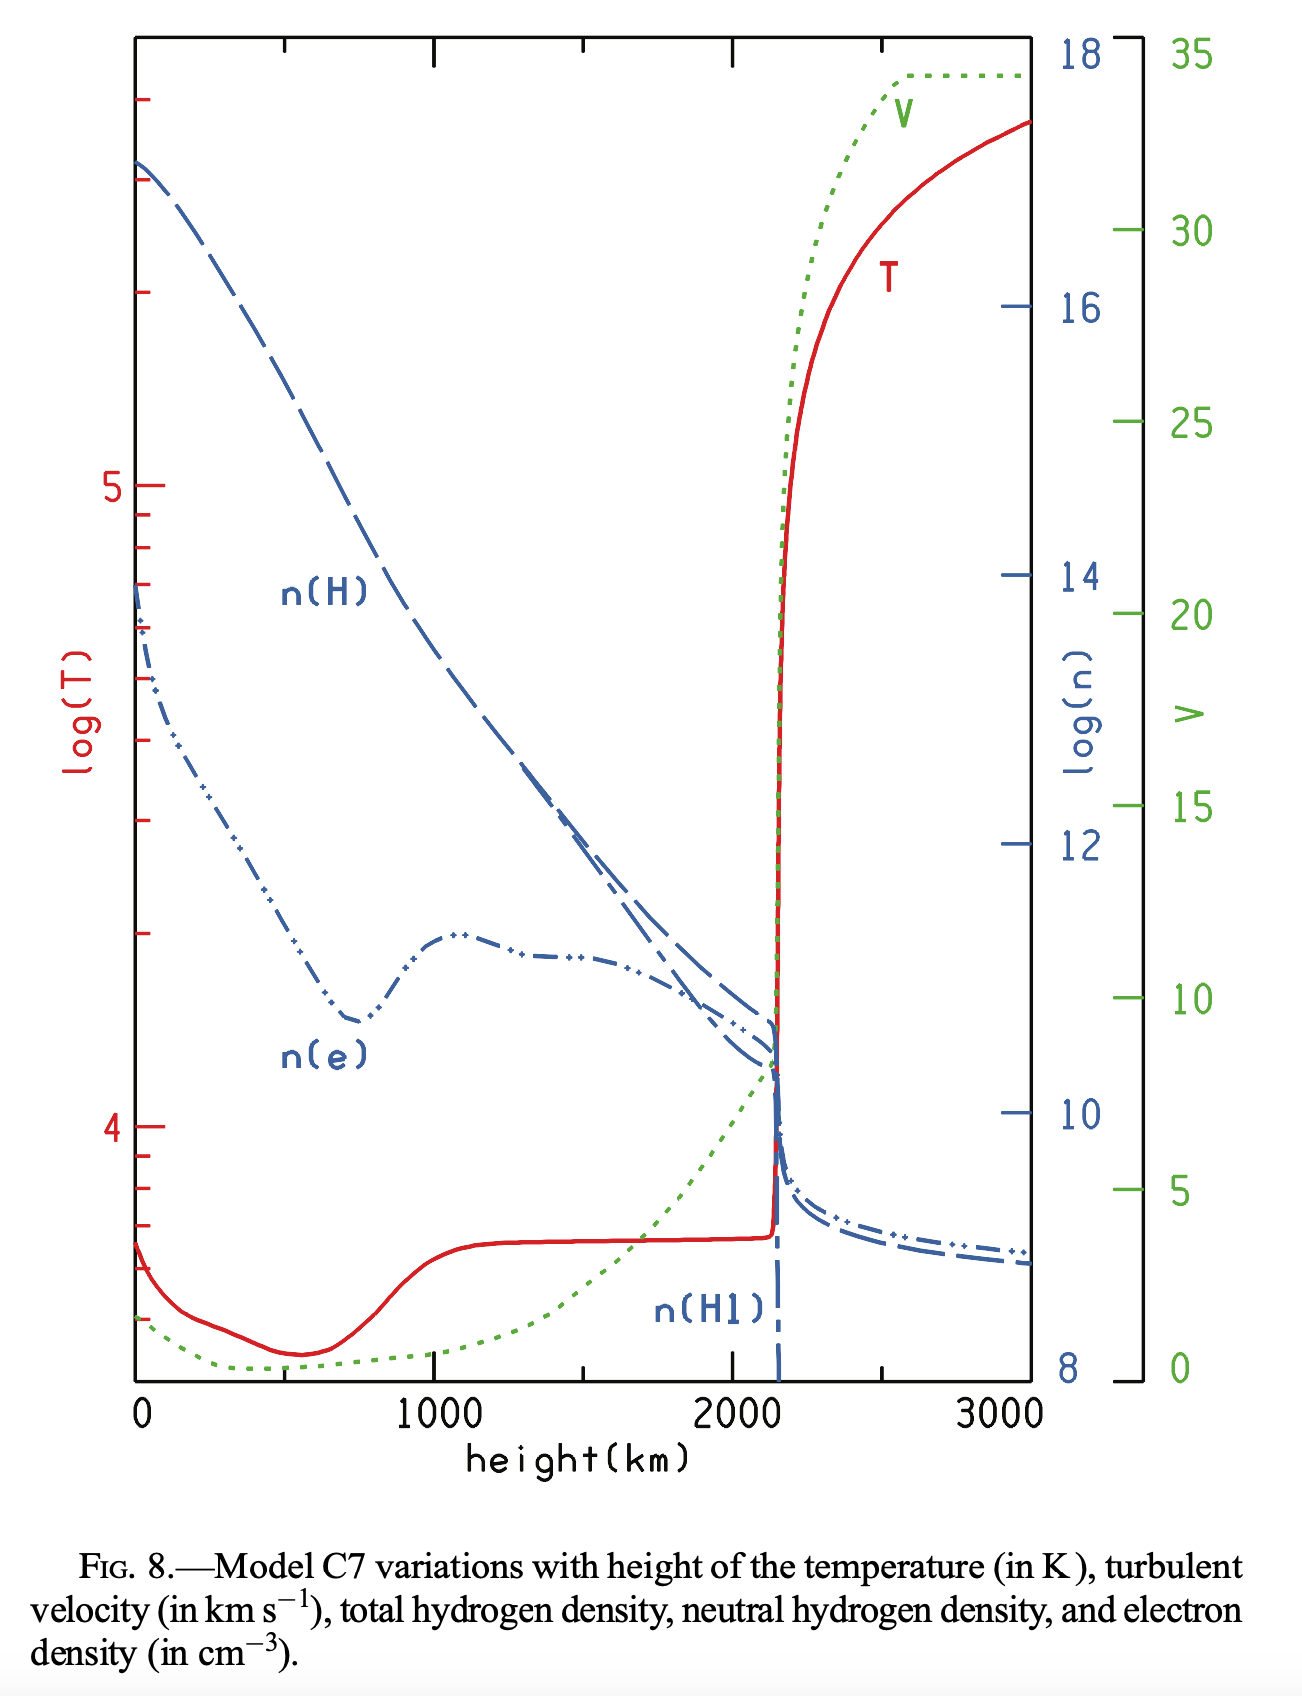
\includegraphics[width=0.65\linewidth]{c7_profile.png}
\end{center}
\figcap{\textbf{Model C7 atmosphere} \parencite{AvrettLoeser2008} --- the initial state.}
\end{block}

\begin{block}{Physically grounded boundary conditions}
The \mz{photosphere} is a closed $V{=}0$ wall; the \mz{top} is an open outflow
--- a hydrostatic atmosphere stays at rest while the conduction-driven upflow
escapes, neither swamped nor reflected by the boundary.
\textbf{Lower BC --- photosphere:}
\begin{compactitem}
  \item \mz{Discrete-hydrostatic ghost} enforces $dp/ds=-\rho g$ on the actual grid.
  \item Base density \& temperature pinned to Model~C7; $V{=}0$ \parencite{Pandey2024}.
\end{compactitem}
\textbf{Upper BC --- fixed $22$\,kK lower-TR reservoir ($h\approx2.15$\,Mm):}
\begin{compactitem}
  \item The resolved chromosphere+TR ends at the natural $22$\,kK level; a
        \mz{fixed-$T$ ghost} there stands in for the hot atmosphere above.
  \item Its \rd{downward conductive flux} $q\propto(T_\mathrm{ghost}-T_\mathrm{top})$
        \emph{alone} drives the evaporation, and \mz{self-limits} as the top heats
        toward $22$\,kK --- no positive-feedback blow-up.
  \item Hydrostatic ghost pressure (no spurious boundary force) + EOS-consistent
        density; \mz{zero-gradient (Neumann) velocity} so the upflow leaves freely.
\end{compactitem}
\end{block}

\begin{block}{Numerical methods}
Finite-volume on the field line; $B$ as a geometric factor:
\begin{eqbox}
\centering
$\dfrac{\partial \mathbf U_i}{\partial t}=
  -\dfrac{B_i}{\Delta s_i}\!\left(\dfrac{\mathbf F_{i+\frac12}}{B_{i+\frac12}}
  -\dfrac{\mathbf F_{i-\frac12}}{B_{i-\frac12}}\right)+\mathbf S_i$
\end{eqbox}
\begin{compactitem}
  \item \mz{Space:} TVD--MUSCL limited-linear reconstruction $\to$ 2nd order. The
        minmod limiter acts on \mz{$\log\rho$ and $\log p$} (the exponentially-stratified,
        positive slots; $V$ stays linear).
  \item \mz{Flux:} Rusanov (local Lax--Friedrichs).
  \item \mz{Time:} 2-stage Runge--Kutta $\to$ 2nd order.
  \item \mz{Stiff sources} via \mz{Lie} (sequential, first-order) operator splitting,
        each advanced by the full $\Delta t$:
        transport $\Rightarrow$ drag $\Rightarrow$ $T_i$--$T_n$ equilibration $\Rightarrow$
        conduction (Thomas) $\Rightarrow$ ionization (cell quadratic) $\Rightarrow$
        cooling (backward-Euler, positivity-preserving).
\end{compactitem}
\begin{center}
  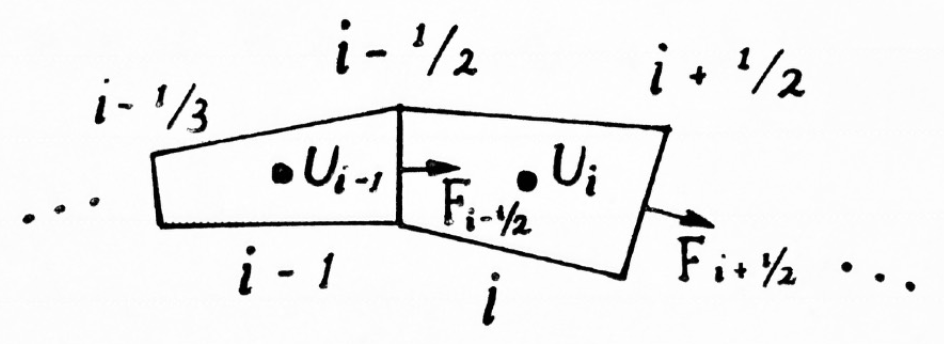
\includegraphics[width=0.68\linewidth]{fv_stencil.png}
\end{center}
\figcap{\textbf{Finite-volume stencil:} cell-averaged states $\mathbf U_i$ updated by
  interface fluxes $\mathbf F_{i\pm1/2}$ along the field line.}
\end{block}

\end{column}
\separatorcolumn

%%=====================================================================
%%  COLUMN 3
%%=====================================================================
\begin{column}{\colwidth}

\begin{block}{Result 1 --- Ionization \& recombination in C7}
\begin{center}
  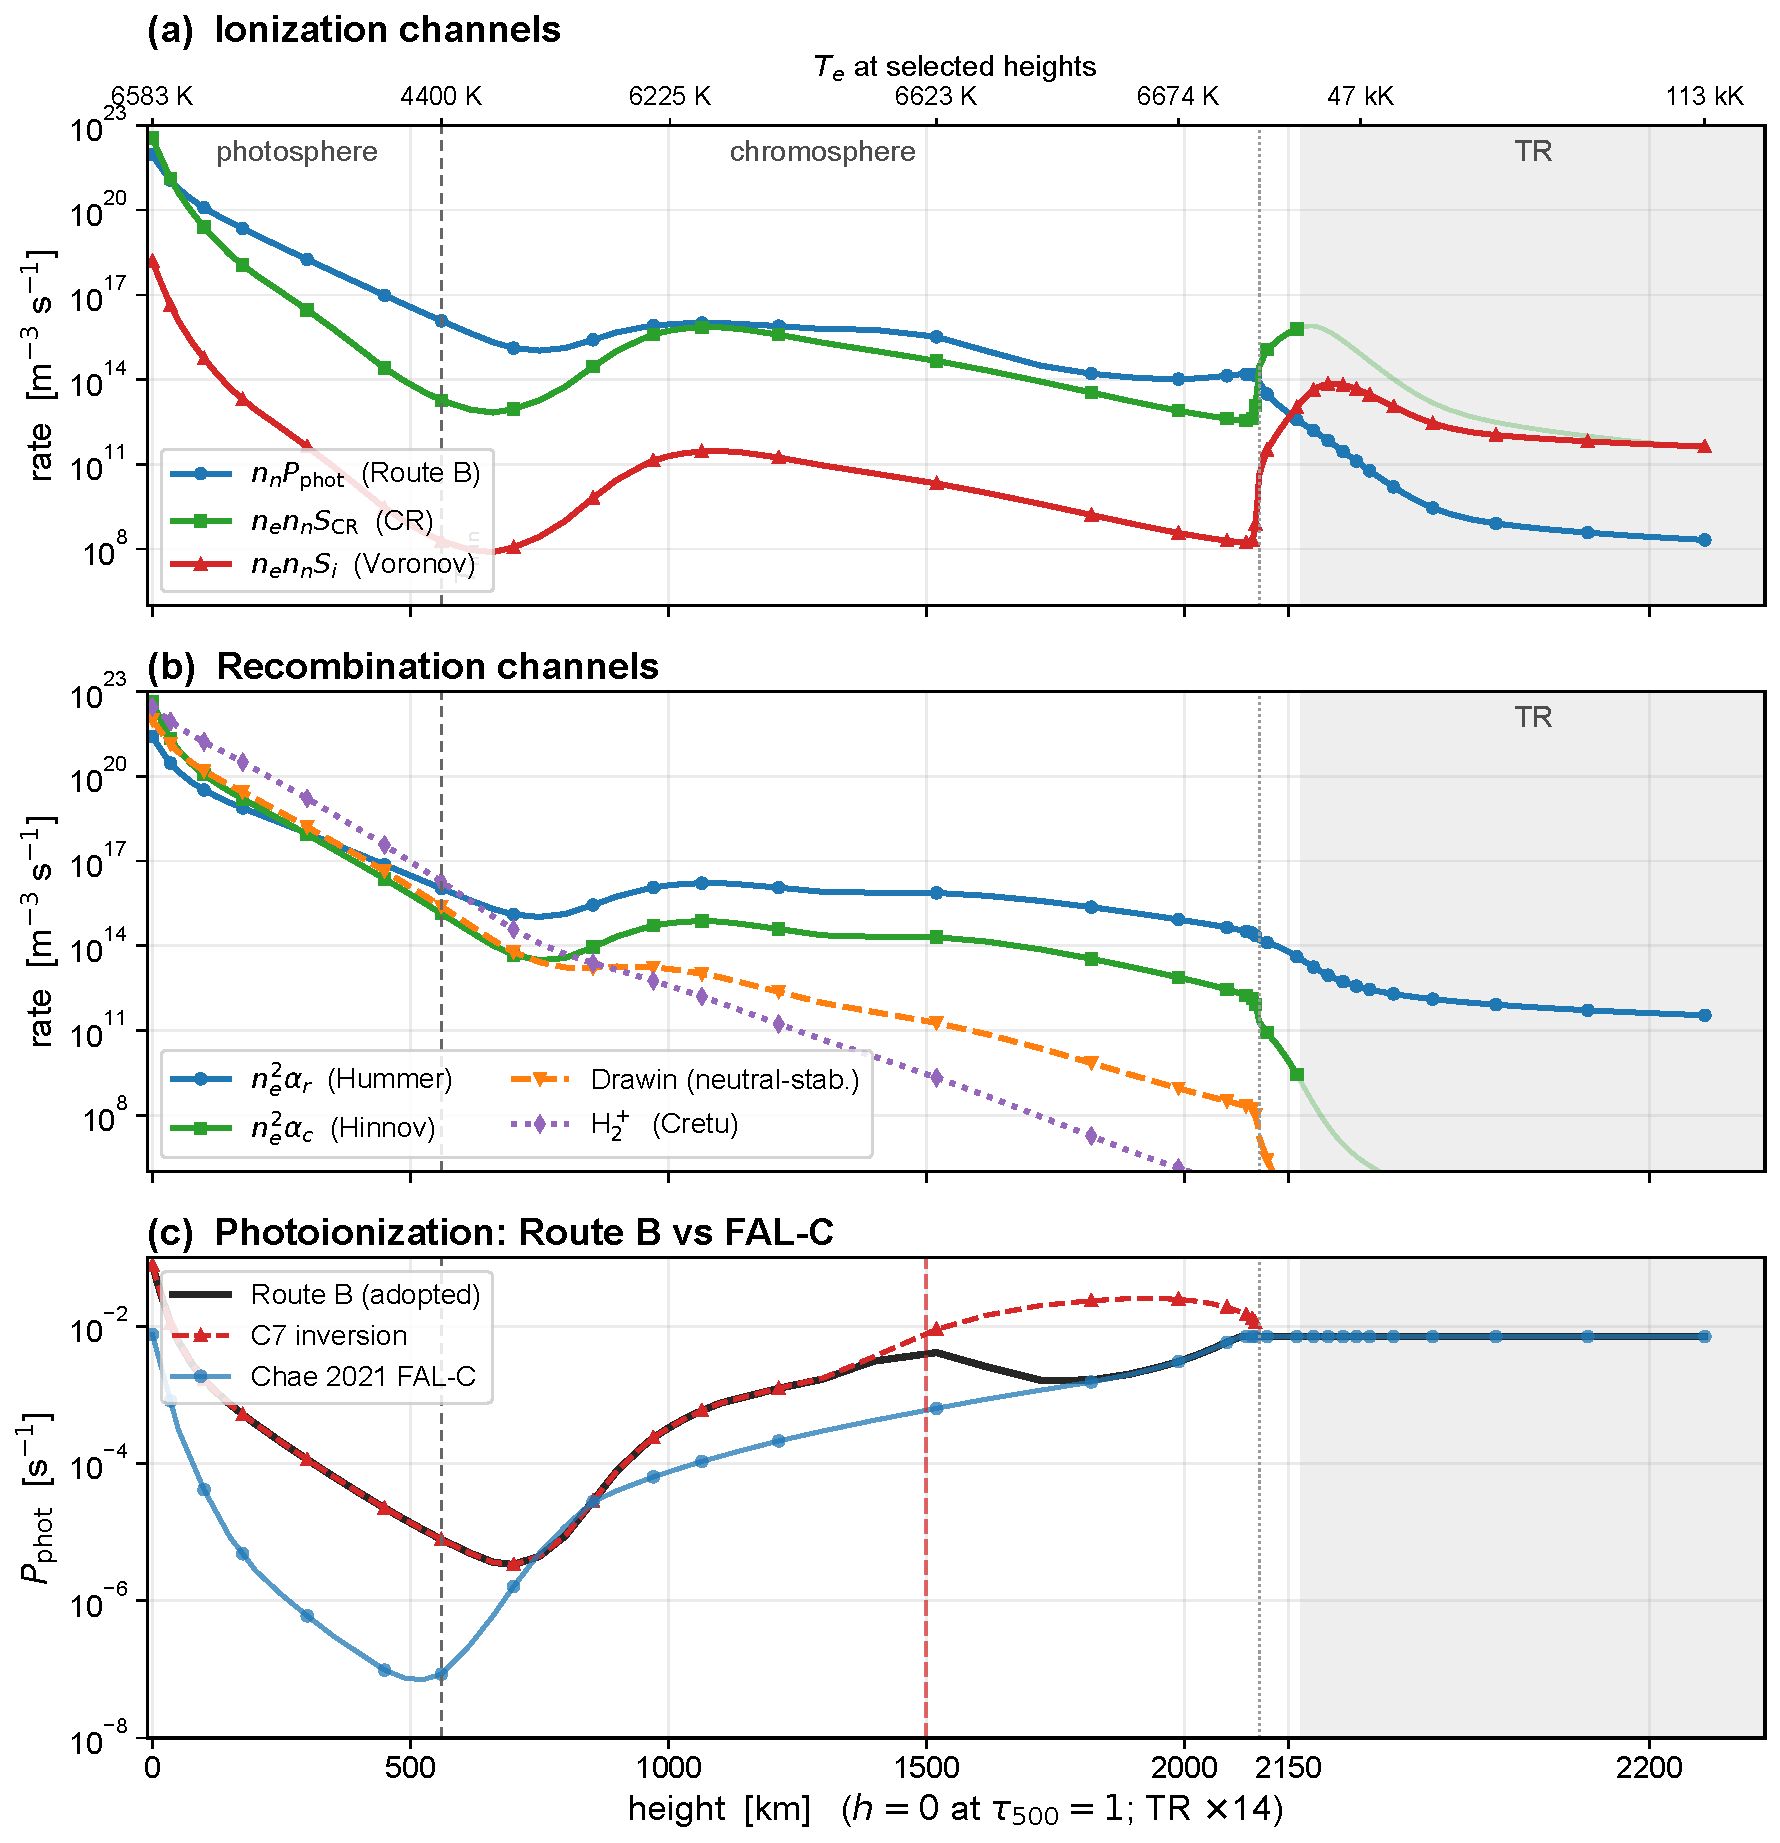
\includegraphics[width=0.98\linewidth]{c7_rates.pdf}
\end{center}
\figcap{\textbf{Dense base:} the collisional pair ($S_{\mathrm{CR}},\alpha_c\propto n_e$)
  dominates (Saha-like). \textbf{Mid/upper chromosphere:} photoionization + radiative
  recombination. \textbf{TR:} direct collisional $S_i$. The frozen radiative-rate
  closure matches FAL-C above $1500$\,km; column cooling $\approx6.6$\,kW\,m$^{-2}$ ($\sim$$10\%$ of the
  CL2012 Bifrost benchmark).}
\end{block}

\begin{block}{Result 2 --- Gentle (conduction-driven) evaporation}
A \mz{first-principles testbed}: the \textbf{real Model-C7 atmosphere} from the
photosphere up to the \textbf{$22$\,kK lower-TR base} ($h=0\to2.15$\,Mm), density
rebuilt hydrostatically, with frozen ionization. Conduction runs from a hydrostatic
$V{=}0$ start --- \rd{no beam, no ad-hoc heating} --- so the \rd{resolved TR's own
downward heat flux} \emph{alone} drives the flow. As this conduction-only testbed has
\rd{no radiative sink}, we set a reduced \mz{$\gamma=1.05$} (near-isothermal;
$c_v{=}k/(\gamma{-}1)\!\to\!\infty$) as a polytropic stand-in for it --- the gas
absorbs the conductive heat at \mz{nearly constant $T$} instead of running away.
\mz{Grid-converged} (ns $=1000/2000/4000$).
\begin{center}
  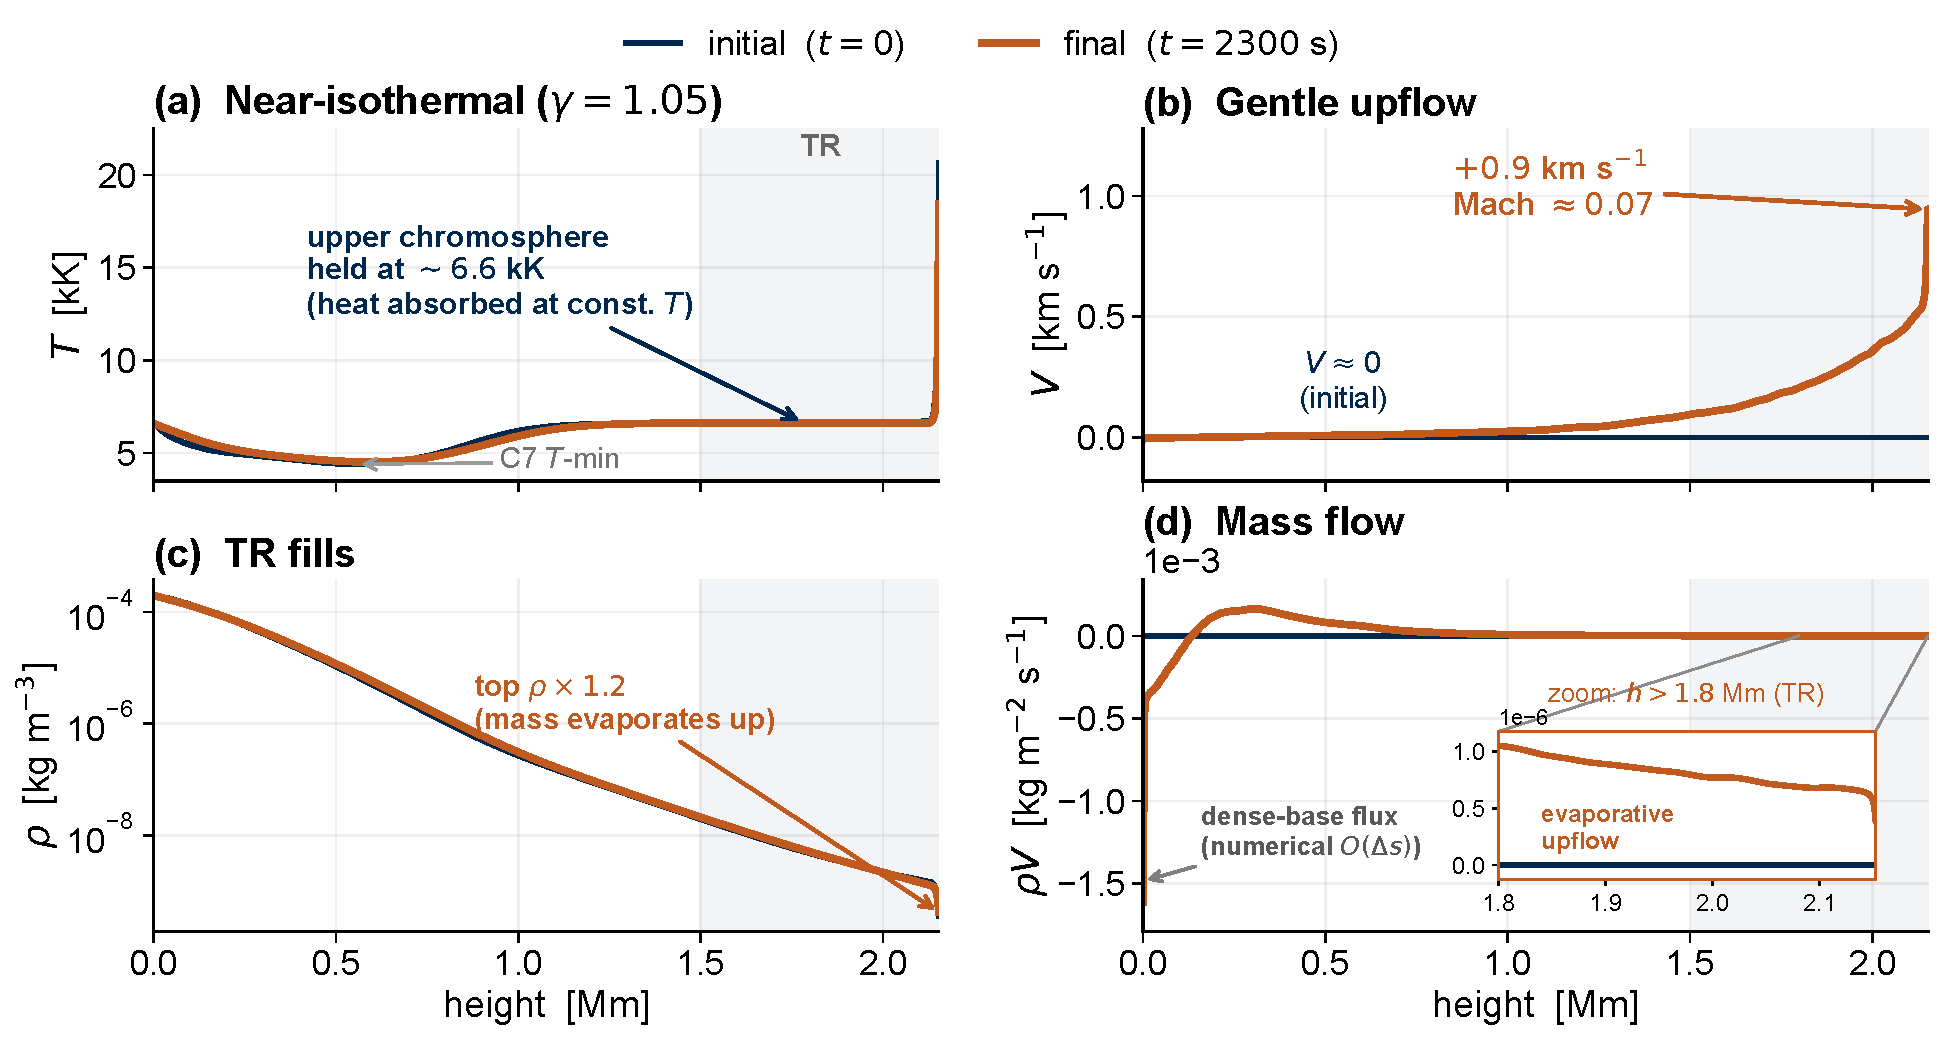
\includegraphics[width=\linewidth]{iso_t22k_snapshots.pdf}
\end{center}
\figcap{\textbf{Initial ($t{=}0$, navy) vs.\ final ($t{\approx}2300$\,s, orange).}
  \textbf{(a)} the upper chromosphere is \mz{held near-isothermal} at $\sim6.6$\,kK ---
  conductive heat absorbed at constant $T$; \textbf{(b)} a gentle $+0.95$\,km/s upflow
  develops at the TR (Mach $\approx0.07$ --- deeply subsonic); \textbf{(c)} the TR/top
  fills modestly ($\sim1.2\times$); \textbf{(d)} the \emph{whole}-column mass flux
  $\rho V$ --- the dense base carries a large \rd{numerical $O(\Delta s)$} drainage
  spike --- with a \mz{zoom on $h>1.8$\,Mm}, where the grid-converged evaporative
  upflow ($\sim\!10^{-6}$) lives. Single linear height axis; the upper-chromosphere\,+\,TR
  region is shaded.}
\vspace{0.2ex}
\begin{center}\small
\begin{tabular}{lcc}
\toprule
\textbf{Quantity} & \textbf{Initial} & \textbf{Evaporating}\\
\midrule
Upper-chromo.\ $T$ ($h\!\approx\!1.8$\,Mm) & $6.7$\,kK & \evap{$6.6$\,kK (held)}\\
Peak upflow $V$                           & $0$       & \evap{$+0.95$\,km/s}\\
Upflow Mach                               & ---       & \evap{$\approx0.07$ (subsonic)}\\
TR/top density                            & $1\times$ & \evap{$\sim1.2\times$}\\
\bottomrule
\end{tabular}
\end{center}
\vspace{0.1ex}
Deeply subsonic upflow $\Rightarrow$ \emph{gentle} evaporation
\parencite{AntiochosSturrock1978}, recovered from \mz{conduction alone} and
\mz{near-isothermal} under the
$\gamma{=}1.05$ closure that stands in
for the radiative sink. A self-consistent radiative sink and a resolved corona above
are the next step toward a sustained quasi-steady state.
\end{block}

\begin{block}{Conclusions \& outlook}
\begin{hlbox}
A self-consistent, dynamic chromosphere that \mz{solves} the lower boundary AWSoM-R
currently prescribes.
\end{hlbox}
\begin{compactitem}
  \item A field-aligned \mz{two-fluid} model: non-equilibrium H ionization, multi-channel
        radiative cooling, physical coronal BC --- run along \mz{PFSS field lines}.
  \item Recovers chromospheric ionization structure \emph{and} the gentle
        conduction-driven evaporation signature (EM rise, subsonic upflow, TR burndown).
  \item Designed as a \rd{drop-in dynamic lower boundary for AWSoM-R}.
  \item \textbf{Next:} two-way coupling into SWMF; PFSS-line ensembles for full events.
\end{compactitem}
\begin{center}
  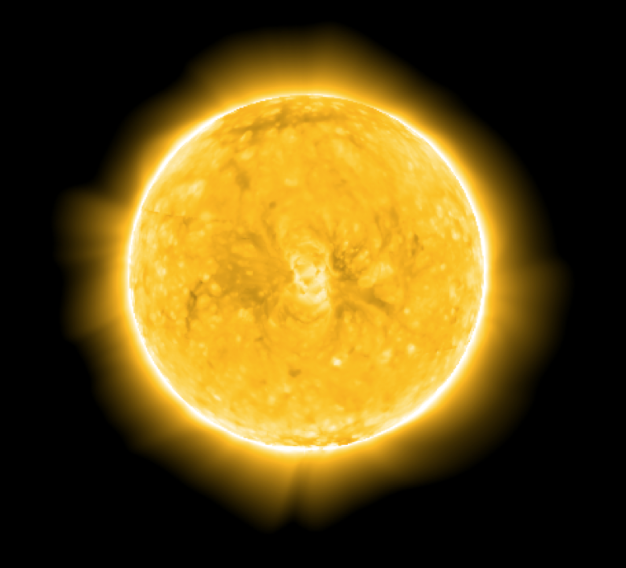
\includegraphics[height=7.4cm]{synth_aia171.png}\hspace{0.7cm}
  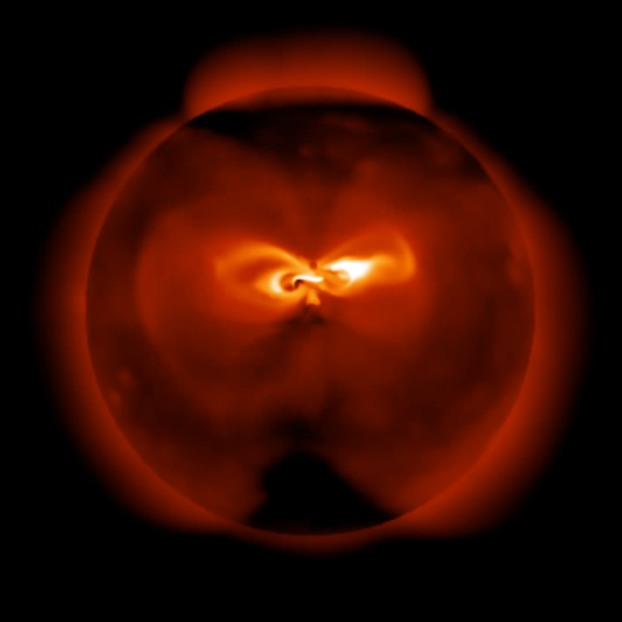
\includegraphics[height=7.4cm]{synth_xray_cme.png}
\end{center}
\figcap{\textbf{Downstream science enabled:} synthetic AIA\,$171$\,\AA\ of a global
  coronal model (left) and a synthetic X-ray CME (right).}
\end{block}

\begin{block}{Acknowledgements \& key references}
\footnotesize
Supported by the NASA Space Weather Center of Excellence \mz{CLEAR} (80NSSC23M0191) and
the SWMF effort at the University of Michigan.\\[2pt]
% RTV (coronal scaling) and Johnston (TRAC) are key method references kept in the list.
\nocite{RosnerTuckerVaiana1978,Johnston2020}
\begin{multicols}{2}
\printbibliography[heading=none]
\end{multicols}
\end{block}

\end{column}
\separatorcolumn
\end{columns}
\end{frame}
\end{document}
